\section{密度}\label{sec:4-1}

我们周围有各种物质,例如空气、水、泥土、石头、铁、铜等等,每种物质都有各自的特性。
空气是气体,水是液体;泥土是松的,石头是硬的;铁是银白色的,铜是紫红色的,我们就是根据物质的特性来辨认它们的。
物质除了具有形态、颜色、软硬等特性外,还有其它的特性。
例如,铁和铝虽然都是金属,都很硬,颜色也差不多,但是如果把体积相等的铁块和铝块放在天平上,
可以看出它们的质量是不相等的(图 \ref{fig:4-1}),铁块的质量大,铝块的质量小。
水和酒精都是透明的液体,但是体积相等的水和酒精的质量也不相等(图 \ref{fig:4-2}),水的质量大,酒精的质量小。
在体积相等的情况下,不同物质的质量不同,也是物质的一种特性。
在物学里里,用\textbf{密度}这个物理量来表示这种特性。


\begin{figure}[htbp]
    \centering
    \begin{minipage}{7cm}
    \centering
    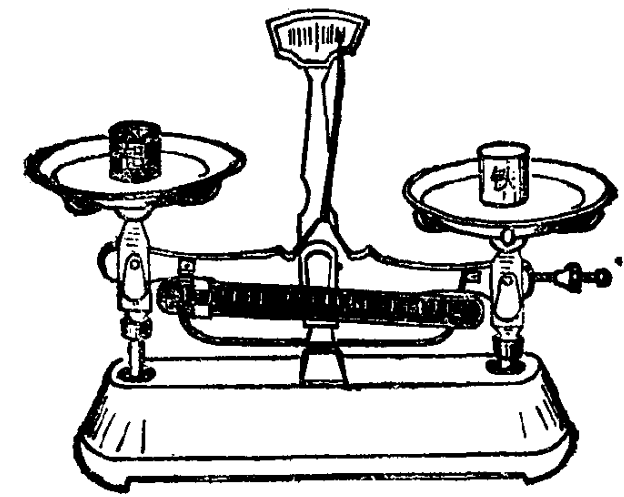
\includegraphics[width=7cm]{../pic/czwl1-ch4-1}
    \caption{体积相等的铁块和铝块质量不相等}\label{fig:4-1}
    \end{minipage}
    \qquad
    \begin{minipage}{7cm}
    \centering
    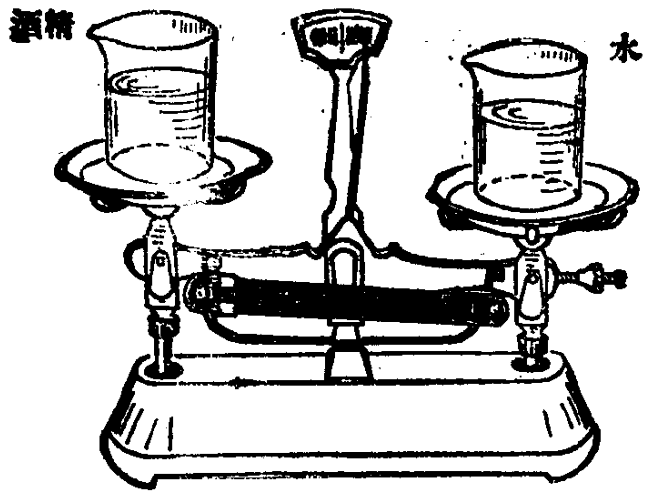
\includegraphics[width=7cm]{../pic/czwl1-ch4-2}
    \caption{体积相等的水和酒精质量不相等}\label{fig:4-2}
    \end{minipage}
\end{figure}

\textbf{单位体积的某种物质的质量,叫做这种物质的密度}。

在国际单位制中,质量的主单位是千克,体积的主单位是立方米,于是取 1 立方米物质的质量作为物质的密度。
例如,$3 \lfm$ 铁的质量是 $2.34 \times 10^4$ 千克,铁的密度就是
$$ \dfrac{2.34 \times 10^4 \text{千克}}{3 \lfm} = 7.8 \times 10^3 \; \qkmlfm \; \text{。} $$

可见,计算密度的公式是
$$ \text{密度} = \dfrac{\text{质量}}{\text{体积}} \; \text{。} $$

如果用 $\rho$ \, \footnote{$\rho$:希腊字母,汉语拼音读法是 rou 。} 代表密度,
$m$ 代表质量,$V$ 代表体积,那么上面的公式可以写作
$$ \rho = \dfrac{m}{V} \; \text{。} $$

从上面的计算可以看出,密度的单位是$\qkmlfm$,读作“千克每立方米”,意思是每立方米多少千克。
例如,铁的密度是 $7.8 \times 10^3 \qkmlfm$ , 读作“$7.8 \times 10^3$ 千克每立方米”,
意思是每立方米铁的质量是 $7.8 \times 10^3$ 千克。

密度的单位也可以用$\kmlflm$。如果质量的单位用克,体积的单位用$\lflm$,密度的单位就是$\kmlflm$。由于
$$ 1 \qkmlfm = \dfrac{1000\text{克}}{(100\lflm} = 0.001 \kmlflm \; \text{,} $$
所以物质的密度用 $\qkmlfm$ 和 $\kmlflm$ 作单位时,其数值相差 $1000$ 倍。
例如,水的密度用 $\qkmlfm$ 作单位时是 $1000 \qkmlfm$,
而用 $\kmlflm$ 作单位时,就是 $1 \kmlflm$。

密度是物质的一种特性,每种物质都有一定的密度,例如金的密度是 $19.3 \times 10^3 \qkmlfm$,
铝的密度是 $2.7 \times 10^3 \qkmlfm$ 。

\begin{table}[H]
    \centering
    \caption*{\large\textbf{一些固体的密度}}
    \renewcommand\arraystretch{1.2}
    \begin{tabular}{|w{c}{6em}|w{c}{8em}||w{c}{6em}|w{c}{8em}|}
        \hline
        物质    & 密度($\qkmlfm$)     & 物质      &  密度($\qkmlfm$) \\ \hline
        铂      & $21.5 \times 10^3$    & 大理石    & $2.7 \times 10^3$ \\ \hline
        金      & $19.3 \times 10^3$    & 花岗岩    & $2.6 \times 10^3$ \\ \hline
        铅      & $11.3 \times 10^3$    & 玻璃      & $2.5 \times 10^3$ \\ \hline
        银      & $10.5 \times 10^3$    & 混凝土    & $2.2 \times 10^3$ \\ \hline
        铜      & $8.9 \times 10^3$     & 砖        & $1.4 \text{~} 1.6 \times 10^3$ \\ \hline
        钢、铁  & $7.8 \times 10^3$     & 冰        & $0.9 \times 10^3$ \\ \hline
        铸铁    & $7.0 \times 10^3$     & 蜡        & $0.9 \times 10^3$ \\ \hline
        铝      & $2.7 \times 10^3$     & 干松木    & $0.4 \times 10^3$ \\ \hline
    \end{tabular}
\end{table}

\begin{table}[H]
    \centering
    \caption*{\large\textbf{一些液体的密度}}
    \renewcommand\arraystretch{1.2}
    \begin{tabular}{|w{c}{6em}|w{c}{8em}||w{c}{6em}|w{c}{8em}|}
        \hline
        物质    & 密度($\qkmlfm$)     & 物质      &  密度($\qkmlfm$) \\ \hline
        水银    & $13.6 \times 10^3$    & 柴油      & $0.85 \times 10^3$ \\ \hline
        硫酸    & $1.8 \times 10^3$     & 煤油      & $0.8 \times 10^3$ \\ \hline
        海水    & $1.03 \times 10^3$    & 酒精      & $0.8 \times 10^3$ \\ \hline
        纯水    & $1.0 \times 10^3$     & 汽油      & $0.71 \times 10^3$ \\ \hline
    \end{tabular}
\end{table}


\begin{table}[H]
    \centering
    \caption*{\large\textbf{一些气体的密度}\footnotemark}
    \renewcommand\arraystretch{1.2}
    \begin{tabular}{|w{c}{6em}|w{c}{8em}||w{c}{8em}|w{c}{8em}|}
        \hline
        物质    & 密度($\qkmlfm$) & 物质      &  密度($\qkmlfm$) \\ \hline
        氯      & $3.21$    & 一氧化碳  & $1.25$ \\ \hline
        二氧化碳& $1.98$    & 水蒸气($100\celsius$时) & $0.60$ \\ \hline
        氧      & $1.43$    & 氦    & $0.18$ \\ \hline
        空气    & $1.29$    & 氢    & $0.09$ \\ \hline
    \end{tabular}
\end{table}
\footnotetext{气体的密度跟温度等条件有关系,表中是在通常条件下的密度值。}


\lianxi

(1) 查查密度表,举出两种密度比水小的固体,一种密度比铁大的液体,两种密度比空气小得多的气体。

(2) 有人说把一块铁分成相等的两块,铁的密度就减小一半。这种说法对吗?

(3) 两个金属球的质量相等,体积不相等,哪个球的密度大?

(4) 有一块金属,质量是 6750 千克,体积是 $2.5 \lfm$,这块金属的密度是多少?这是一块什么金属?

(5) 有一满瓶油,油和瓶总的质量是 1.46 千克。已知瓶的质量是 0.5 千克,瓶的容积是 $1.2\text{分米}^3$。求油的密度。

